\documentclass[11pt]{article}
\usepackage{geometry}
\geometry{letterpaper, margin=1in}
\usepackage[utf8]{inputenc}
\usepackage{graphicx}
\usepackage{upgreek}
\usepackage{url}
\usepackage[T1]{fontenc}
\usepackage{amsmath}
\usepackage{hyperref}
\usepackage[colorinlistoftodos]{todonotes}
\usepackage[
backend=biber,
style=ieee,
sorting=none
]{biblatex}
 
\addbibresource{assign.bib}

\title{ECE532S Digital Systems Design \\ \vspace{0.4cm}
       \Large Lab Test 2 Description - Group Demo Project \\ \vspace{0.4cm}
       \small Last Updated: July, 2019}
\author{ }
\date{ }

\begin{document}
\maketitle
\vspace{-1cm}

The purpose of this test project/demo is to understand and integrate some of the components that you will require in your projects. You will learn to connect your Nexys board to an Ethernet network, construct and integrate an IP as well as perform on-chip hardware debugging. In advance of your demonstration in the lab, you should have all of the functionality described below complete and ready to demonstrate. This project is explicitly structured as a group project, you should work on it together.

This is worth XX\% of your final grade. If you do not have the project prepared in advance of your demonstration period, you will be assigned a grade of 0\%. Please ensure that you have signed up for a demo slot or that a TA has informed you of when you are expected to present.




\section{Background and Resources}
\label{sec:back}
The lightweight TCP/IP project (LwIP) is a small implementation of the TCP/IP stack designed to use minimal memory resources.
This stack is well suited for the MicroBlaze processor and Xilinx has incorporated in SDK a version of LwIP that supports the Xilinx Ethernet IP blocks.
To construct an example system that implements an echo server on the Nexys 4 DDR board, follow the steps in the
\href{https://reference.digilentinc.com/learn/programmable-logic/tutorials/nexys-4-ddr-getting-started-with-microblaze-servers/start}{\color{blue}Digilent Tutorial}.
The constructed system will have several major components (DDR memory interface, UART and Ethernet) that can be used as a good starting point for building the design for your course project.
Note that the tutorial implements a server, while you will have to implement a TCP client for this project.
For more information on LwIP, consult the \href{http://lwip.wikia.com/wiki/LwIP_Wiki}{\color{blue}Wiki}, especially the section on the \href{http://lwip.wikia.com/wiki/Raw/TCP}{\color{blue}RAW API} used in the tutorial.

The second new feature that you will make use of in this assignment is the hardware debugger.
\href{https://www.xilinx.com/support/documentation/ip_documentation/ila/v6_2/pg172-ila.pdf}{\color{blue}Chipscope ILA}. A tutorial of an example can be found in \href{https://www.xilinx.com/support/documentation/sw_manuals/xilinx2017_2/ug936-vivado-tutorial-programming-debugging.pdf}{\color{blue}Debugging Tutorial}. Lab 1, 2 and 9 refer to three different ways to add chipscope to your design (append the netlist, add to verilog or add the ILA ip in your design). Finally, for more general information on the board, refer to the Nexys 4 DDR \href{https://reference.digilentinc.com/reference/programmable-logic/nexys-4-ddr/reference-manual}{\color{blue}reference manual}.





\section{What to Do}
\label{sec:instr}
As a group, you are to construct an FPGA hardware system that acts as a network TCP/IP client to a computer server.
Within your hardware system you must include a custom AXI Lite IP component that reads the board switches and buttons, and performs some basic manipulation on these input values.

The system as a whole is reactive to two of the buttons on the Nexys 4 DDR board, and performs its operation in two phases.
\\
\\

\begin{itemize}
\item Phase 1
\begin{itemize}
\item A \emph{transmission} operation is started when \verb|BTNL| is first pressed on the board.
\item Once the button is pressed, the 16 switch values are read and stored as the lower two bytes of a 4-byte word.
\item When \verb|BTNL| is pressed a second time, the value corresponding to the position of the 16 switches on the board is read again and stored as the upper two bytes of the word.
\item Once the 4 bytes that form a word have been received, their value will be inverted by the module. For example, \(01010101010101010000000000000000 \Rightarrow 10101010101010101111111111111111\) 
\item At this stage, your custom IP should signal to the MicroBlaze that a new valid word is ready.
\item The software running on this soft processor will read the full word, establish a TCP/IP connection to the computer server and send the word over the Ethernet network.
\end{itemize}
\item Phase 2
\begin{itemize}
\item A \emph{receive} operation is started when \verb|BTNR| is pressed.
\item Now the MicroBlaze will connect to the computer server and read the current 4-byte word.
\item The retrieved word will be then shown on the 7-segment displays, in hexadecimal.
\end{itemize}

\end{itemize}

A rough block diagram of the main system components is shown in Figure~\ref{fig:blockdiag}.
Supporting IPs have been left out of the diagram for clarity.

\begin{figure}[!b]
\centering
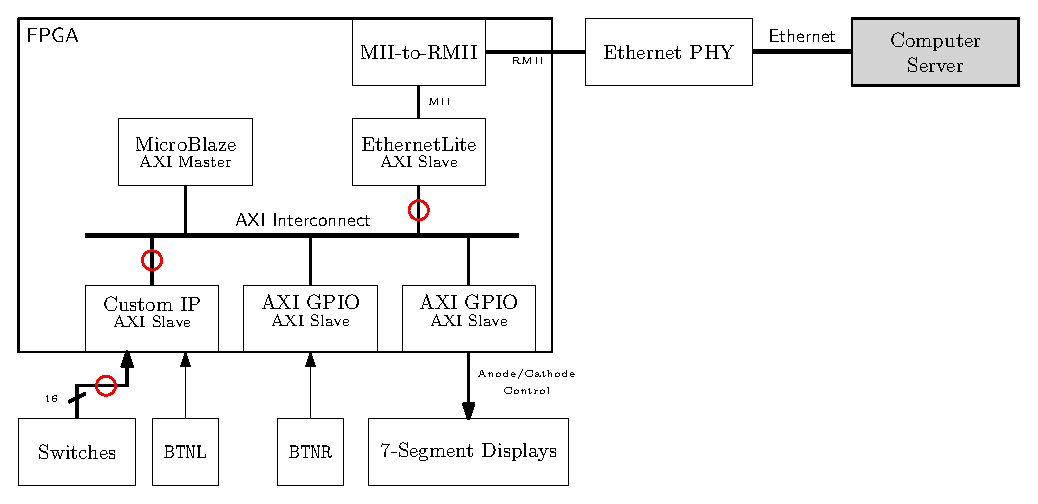
\includegraphics{diag.eps}
\caption{Block diagram of the main system in the warmup project. Red circles indicate hardware probe points explained in Sec.~\ref{sec:wtd:hwdbg}}
\label{fig:blockdiag}
\end{figure}

\subsection{Detailed Specifications}

When a connection is made to the server, one of two commands is expected.
A \verb|GET| command will cause the server to send a 32-bit value corresponding to the value stored in the server.
On the other hand, a \verb|POST| command will update the 32-bit value.
The \verb|POST| message must be accompanied immediately with the new value to set.

For example the byte sequence 0x50, 0x4f, 0x53, 0x54, 0xba, 0xad, 0xf0, 0x0d is a valid \verb|POST| sequence.
The first four bytes correspond to the letters \verb|P|, \verb|O|, \verb|S| and \verb|T| when converted to ASCII and the remaining four bytes make up the new value to set 0xBAADF00D.

The Python3 files \verb|echoserver.py| and \verb|echoclient.py| demonstrate simple versions of the server and client.
You may use the server implementation but the client will have to be implemented in the Nexys 4 DDR board.

\subsection{Hardware Debugging}
\label{sec:wtd:hwdbg}

Once the system is complete, you should use the Xilinx hardware debugger to ensure all of the hardware is working as expected.
Specifically, you are required to set up hardware probes at the three interfaces highlighted with red circles in Fig.~\ref{fig:blockdiag}.
You will be asked during the demonstration of your project to trigger transactions at these interfaces and you should be able to explain what is happening.

\section{Tips}

To get this system to work, you will need to connect the Nexys 4 DDR board to a computer with an Ethernet port.
The Nexys 4 DDR Ethernet PHY supports automatic Medium-Dependent Interface Crossover (MDIX), thus a straight or crossover cable can be used to connect the board to a switch or directly your computer.

Python3 must be installed on your personal computer to run the example scripts.
Executing the \verb|echoserver.py| script should start a process listening for incoming TCP/IP connections on port 9090 by default.
The \verb|echoclient.py| connects to the server via the ``localhost" address \verb|127.0.0.1|. 
You may modify the server and client scripts to better suit your environment.


\newpage
\printbibliography

\end{document}
